\documentclass[journal,12pt,twocolumn]{IEEEtran}
\usepackage{setspace}
\usepackage{gensymb}
\usepackage{caption}
%\usepackage{multirow}
%\usepackage{multicolumn}
%\usepackage{subcaption}
%\doublespacing
\singlespacing
\usepackage{csvsimple}
\usepackage{amsmath}
\usepackage{multicol}
%\usepackage{enumerate}
\usepackage{amssymb}
%\usepackage{graphicx}
\usepackage{newfloat}
%\usepackage{syntax}
\usepackage{listings}
%\usepackage{iithtlc}
\usepackage{color}
\usepackage{tikz}
\usetikzlibrary{shapes,arrows}



%\usepackage{graphicx}
%\usepackage{amssymb}
%\usepackage{relsize}
%\usepackage[cmex10]{amsmath}
%\usepackage{mathtools}
%\usepackage{amsthm}
%\interdisplaylinepenalty=2500
%\savesymbol{iint}
%\usepackage{txfonts}
%\restoresymbol{TXF}{iint}
%\usepackage{wasysym}
\usepackage{amsthm}
\usepackage{mathrsfs}
\usepackage{txfonts}
\usepackage{stfloats}
\usepackage{epstopdf}
\usepackage{cite}
\usepackage{cases}
\usepackage{mathtools}
\usepackage{caption}
\usepackage{enumerate}	
\usepackage{enumitem}
\usepackage{amsmath}
%\usepackage{xtab}
\usepackage{longtable}
\usepackage{multirow}
%\usepackage{algorithm}
%\usepackage{algpseudocode}
\usepackage{enumitem}
\usepackage{mathtools}
\usepackage{hyperref}
%\usepackage[framemethod=tikz]{mdframed}
\usepackage{listings}
    %\usepackage[latin1]{inputenc}                                 %%
    \usepackage{color}                                            %%
    \usepackage{array}                                            %%
    \usepackage{longtable}                                        %%
    \usepackage{calc}                                             %%
    \usepackage{multirow}                                         %%
    \usepackage{hhline}                                           %%
    \usepackage{ifthen}                                           %%
  %optionally (for landscape tables embedded in another document): %%
    \usepackage{lscape}     


\usepackage{url}
\def\UrlBreaks{\do\/\do-}


%\usepackage{stmaryrd}


%\usepackage{wasysym}
%\newcounter{MYtempeqncnt}
\DeclareMathOperator*{\Res}{Res}
%\renewcommand{\baselinestretch}{2}
\renewcommand\thesection{\arabic{section}}
\renewcommand\thesubsection{\thesection.\arabic{subsection}}
\renewcommand\thesubsubsection{\thesubsection.\arabic{subsubsection}}

\renewcommand\thesectiondis{\arabic{section}}
\renewcommand\thesubsectiondis{\thesectiondis.\arabic{subsection}}
\renewcommand\thesubsubsectiondis{\thesubsectiondis.\arabic{subsubsection}}

% correct bad hyphenation here
\hyphenation{op-tical net-works semi-conduc-tor}

%\lstset{
%language=C,
%frame=single, 
%breaklines=true
%}

%\lstset{
	%%basicstyle=\small\ttfamily\bfseries,
	%%numberstyle=\small\ttfamily,
	%language=Octave,
	%backgroundcolor=\color{white},
	%%frame=single,
	%%keywordstyle=\bfseries,
	%%breaklines=true,
	%%showstringspaces=false,
	%%xleftmargin=-10mm,
	%%aboveskip=-1mm,
	%%belowskip=0mm
%}

%\surroundwithmdframed[width=\columnwidth]{lstlisting}
\def\inputGnumericTable{}                                 %%
\lstset{
%language=C,
frame=single, 
breaklines=true,
columns=fullflexible
}
 

\begin{document}
%
\tikzstyle{block} = [rectangle, draw,
    text width=3em, text centered, minimum height=3em]
\tikzstyle{sum} = [draw, circle, node distance=3cm]
\tikzstyle{input} = [coordinate]
\tikzstyle{output} = [coordinate]
\tikzstyle{pinstyle} = [pin edge={to-,thin,black}]

\theoremstyle{definition}
\newtheorem{theorem}{Theorem}[section]
\newtheorem{problem}{Problem}
\newtheorem{proposition}{Proposition}[section]
\newtheorem{lemma}{Lemma}[section]
\newtheorem{corollary}[theorem]{Corollary}
\newtheorem{example}{Example}[section]
\newtheorem{definition}{Definition}[section]
%\newtheorem{algorithm}{Algorithm}[section]
%\newtheorem{cor}{Corollary}
\newcommand{\BEQA}{\begin{eqnarray}}
\newcommand{\EEQA}{\end{eqnarray}}
\newcommand{\define}{\stackrel{\triangle}{=}}
\bibliographystyle{IEEEtran}
%\bibliographystyle{ieeetr}
\providecommand{\nCr}[2]{\,^{#1}C_{#2}} % nCr
\providecommand{\nPr}[2]{\,^{#1}P_{#2}} % nPr
\providecommand{\mbf}{\mathbf}
\providecommand{\pr}[1]{\ensuremath{\Pr\left(#1\right)}}
\providecommand{\qfunc}[1]{\ensuremath{Q\left(#1\right)}}
\providecommand{\sbrak}[1]{\ensuremath{{}\left[#1\right]}}
\providecommand{\lsbrak}[1]{\ensuremath{{}\left[#1\right.}}
\providecommand{\rsbrak}[1]{\ensuremath{{}\left.#1\right]}}
\providecommand{\brak}[1]{\ensuremath{\left(#1\right)}}
\providecommand{\lbrak}[1]{\ensuremath{\left(#1\right.}}
\providecommand{\rbrak}[1]{\ensuremath{\left.#1\right)}}
\providecommand{\cbrak}[1]{\ensuremath{\left\{#1\right\}}}
\providecommand{\lcbrak}[1]{\ensuremath{\left\{#1\right.}}
\providecommand{\rcbrak}[1]{\ensuremath{\left.#1\right\}}}
\theoremstyle{remark}
\newtheorem{rem}{Remark}
\newcommand{\sgn}{\mathop{\mathrm{sgn}}}
%\providecommand{\abs}[1]{\left\vert#1\right\vert}
\providecommand{\res}[1]{\Res\displaylimits_{#1}} 
\providecommand{\norm}[1]{\lVert#1\rVert}
\providecommand{\mtx}[1]{\mathbf{#1}}
%\providecommand{\mean}[1]{E\left[ #1 \right]}
\providecommand{\fourier}{\overset{\mathcal{F}}{ \rightleftharpoons}}
%\providecommand{\hilbert}{\overset{\mathcal{H}}{ \rightleftharpoons}}
\providecommand{\system}{\overset{\mathcal{H}}{ \longleftrightarrow}}
	%\newcommand{\solution}[2]{\textbf{Solution:}{#1}}
\newcommand{\solution}{\noindent \textbf{Solution: }}
\newcommand{\myvec}[1]{\ensuremath{\begin{pmatrix}#1\end{pmatrix}}}
\providecommand{\dec}[2]{\ensuremath{\overset{#1}{\underset{#2}{\gtrless}}}}
\DeclarePairedDelimiter{\ceil}{\lceil}{\rceil}
%\numberwithin{equation}{section}
%\numberwithin{problem}{subsection}
%\numberwithin{definition}{subsection}
\makeatletter
\@addtoreset{figure}{section}
\makeatother
\let\StandardTheFigure\thefigure
%\renewcommand{\thefigure}{\theproblem.\arabic{figure}}
\renewcommand{\thefigure}{\thesection}
%\numberwithin{figure}{subsection}
%\numberwithin{equation}{subsection}
%\numberwithin{equation}{section}
%\numberwithin{equation}{problem}
%\numberwithin{problem}{subsection}
\numberwithin{problem}{section}
%%\numberwithin{definition}{subsection}
%\makeatletter
%\@addtoreset{figure}{problem}
%\makeatother
\makeatletter
\@addtoreset{table}{section}
\makeatother
\let\StandardTheFigure\thefigure
\let\StandardTheTable\thetable
\let\vec\mathbf
%%\renewcommand{\thefigure}{\theproblem.\arabic{figure}}
%\renewcommand{\thefigure}{\theproblem}
%%\numberwithin{figure}{section}
%%\numberwithin{figure}{subsection}
\def\putbox#1#2#3{\makebox[0in][l]{\makebox[#1][l]{}\raisebox{\baselineskip}[0in][0in]{\raisebox{#2}[0in][0in]{#3}}}}
     \def\rightbox#1{\makebox[0in][r]{#1}}
     \def\centbox#1{\makebox[0in]{#1}}
     \def\topbox#1{\raisebox{-\baselineskip}[0in][0in]{#1}}
     \def\midbox#1{\raisebox{-0.5\baselineskip}[0in][0in]{#1}}
\vspace{3cm}
\title{ 
%	\logo{
Butterworth Filter and Sallen-Key Topology
%	}
}
\author{ Dheeraj Racha and Utkarsh Bhura $^{*}$% <-this % stops a space
	\thanks{*The author is with the Department
		of Electrical Engineering, Indian Institute of Technology, Hyderabad
		502285 India e-mail:  gadepall@iith.ac.in. All solutions in this manual is released under GNU 
GPL.  Free and open source.}
	
}
\maketitle
\tableofcontents
\bigskip
\renewcommand{\thefigure}{\theenumi}
\renewcommand{\thetable}{\theenumi}
\begin{abstract}
This manual gives an idea about Butterworth filter and its use in signal processing. Sallen-Key topology is used to implement linear analog filter.   
\end{abstract}
\section{Introduction}
\begin{enumerate}[label=\thesection.\arabic*,ref=\thesection.\theenumi]
%\begin{enumerate}[label=\arabic*]
\numberwithin{equation}{enumi}
\item What is a Butterworth Filter?\\
\solution It is a low pass filter designed to have a linear magnitude response in pass band. So, it is also referred to as a maximally flat magnitude filter. Even though it does not provide the sharp cut-off response, it is often considered as the all-round filter which is used in many applications.

\numberwithin{equation}{enumi}
%\begin{figure}[!ht]
%\centering
%\includegraphics[width=\columnwidth]{./figs/Buttergr.jpg}
%\caption{}
%\label{fig:2}
%\end{figure}
\end{enumerate}
\section{Frequency Response}
\begin{enumerate}[label=\thesection.\arabic*,ref=\thesection.\theenumi]
\numberwithin{equation}{enumi}
% \item What can you say about the frequency response of this filter?\\
% \solution The Butterworth filter has frequency response as flat as mathematically possible, hence it is also called as a maximally flat magnitude filter (from 0 Hz to cut-off frequency at -3dB \textbf{without any ripples}).\\
\item Write a mathematical expression for the magnitude response of this filter.\\
\solution
\bigskip
\vspace{-1em} $$ |H_{n}(j\omega)|= \frac{V_{o}}{V_{i}}=\frac{1}{\sqrt{1+{(\frac{\omega}{\omega _c}) ^{2N}}}}$$

 where \textit{$\omega _c $ is the cut-off/corner frequency, $N$ is the order of the filter or number of reactive elements in a passive filter.\\}
\item Plot the frequency response of an ideal Butterworth filter. Write your inference.\\
\solution Refer to Fig.2.2 for frequency response.\\
The Butterworth filter achieves pass band flatness at the expense of a wide transition band as the filter changes from the pass band to the stop band.

\begin{figure}{enumi}
\centering
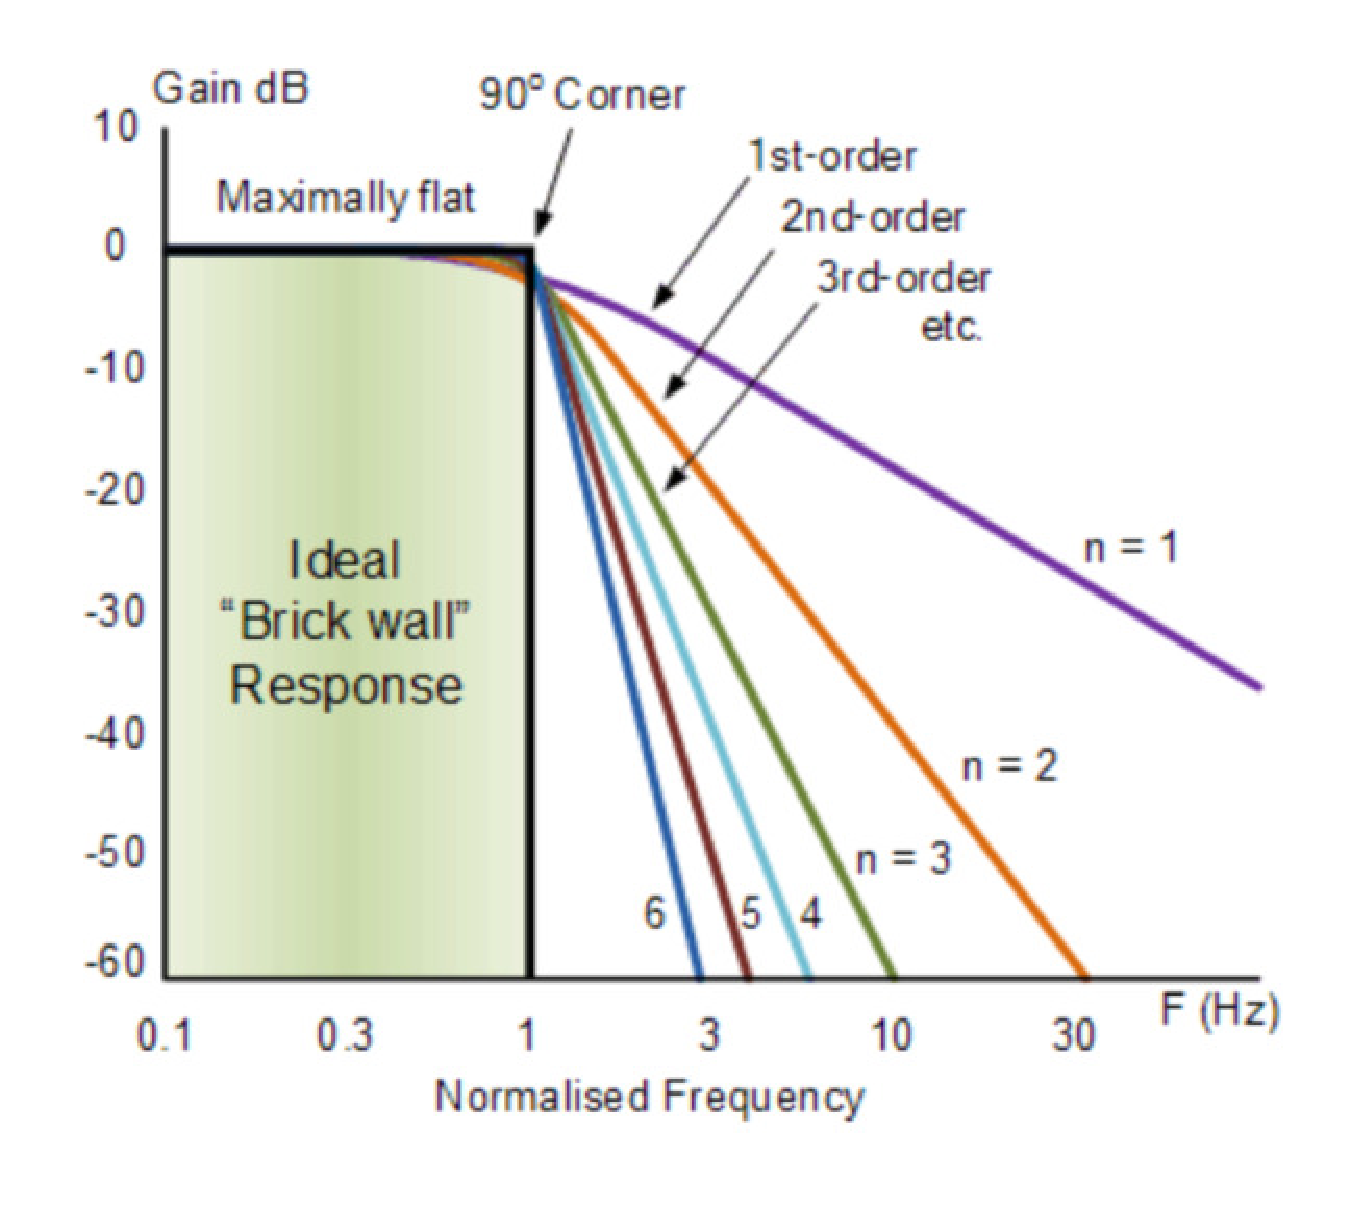
\includegraphics[width=\columnwidth]{./figs/plotforgain.eps}
\caption{}
\label{fig:1}
\end{figure}
\end{enumerate}
\section{Filter Implementation using Circuits}
\begin{enumerate}[label=\thesection.\arabic*,ref=\thesection.\theenumi]
\numberwithin{equation}{enumi}
% \item What is Filter topology?\\
% \solution Electronic filter topology defines electronic filter circuits without taking note of the values of the components used but only the manner in which those components are connected.\\
\item What are the Filter topologies used to implement this filter.\\
\solution There are several different filter topologies available to implement a linear analog filter. The most often used topology for a passive realisation is Cauer topology and the most often used topology for an active realisation is Sallen–Key topology.\\
\item Describe briefly Cauer and Sallen-Key \\ topology. \\
 \solution $(i)$ \textit{{Cauer Topology}}: The Cauer \\ topology uses passive components (shunt capacitors and series inductors) to implement a linear analog filter. The Butterworth filter having a given transfer function can be realised using a Cauer 1-form. Fig shown below is an example of Cauer topology. \\
 \begin{figure}[!ht]
\centering
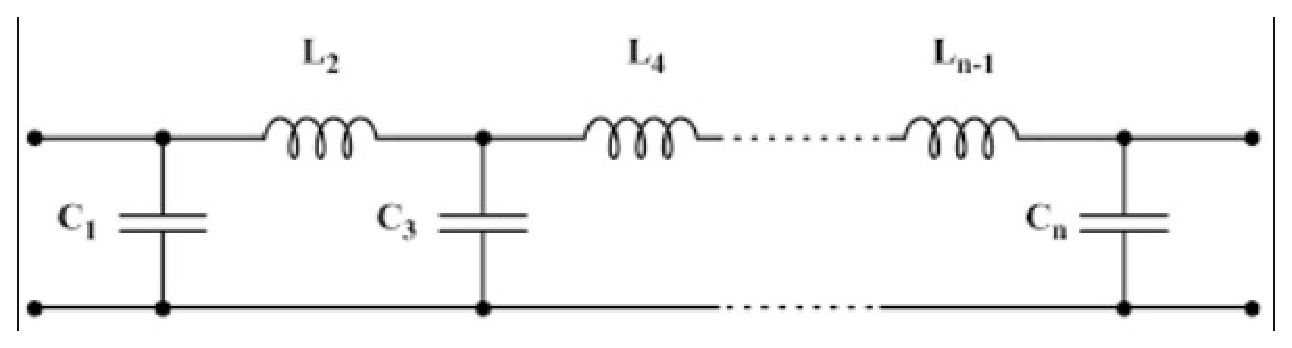
\includegraphics[width=0.7\columnwidth]{./figs/Cauer.eps}
\caption{}
\label{fig:1}
\end{figure}
 $(ii)$ \textit{Sallen-Key Topology}: The Sallen–Key \\ topology uses active and passive components (op-amps operating in non-inverting region, resistors, and capacitors) to implement a linear analog filter. Each Sallen–Key stage implements a conjugate pair of poles; the overall filter is implemented by cascading all stages in series. Fig shown below is an example of Sallen-Key topology.\\
 \begin{figure}[!ht]
\centering
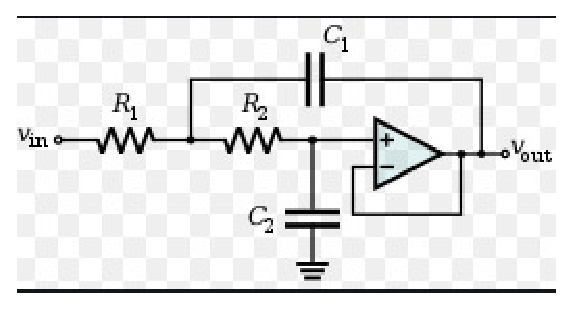
\includegraphics[width=\columnwidth]{./figs/sallenkey.eps}
\caption{A second order sallen-key filter}
\label{fig:2}
\end{figure}
**\textbf{NOTE}: We will limit our discussion to Sallen-Key topology only.
\end{enumerate}

\section{Sallen-Key Circuit Analysis}
\begin{enumerate}[label=\thesection.\arabic*,ref=\thesection.\theenumi]
\item Derive the expression for transfer function of a general second order sallen-key filter.\\
\solution
\begin{figure}[!ht]
\centering
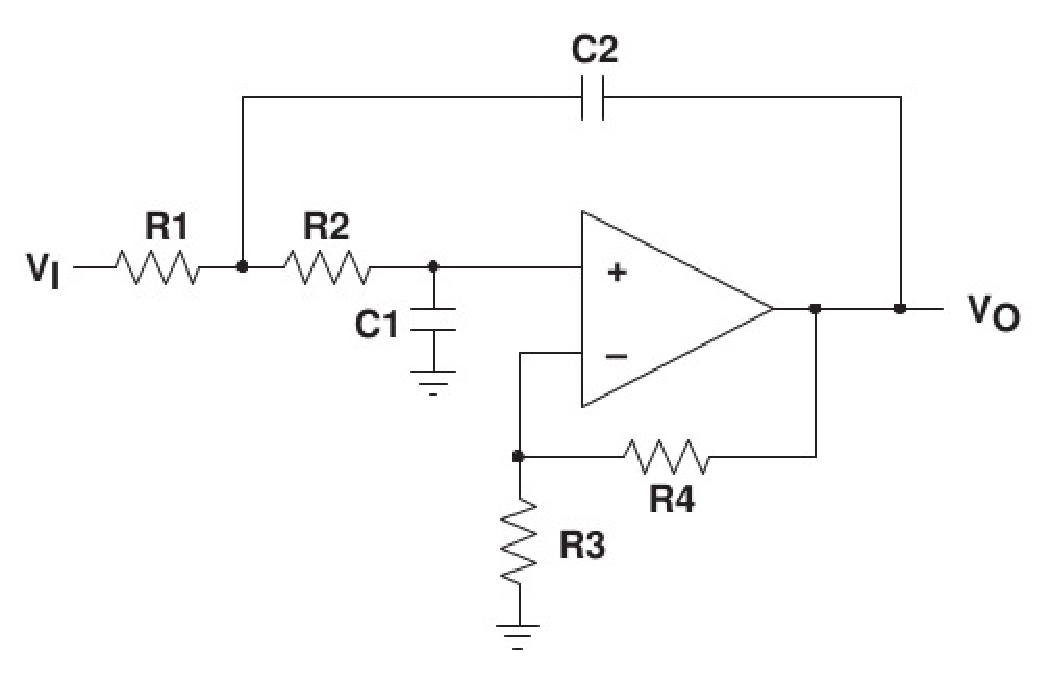
\includegraphics[width=0.7\columnwidth]{./figs/sallen_key_general.eps}
\caption{}
\label{fig:2}
\end{figure}
Because the op-amp is operating in non-inverting region,
\begin{equation}
V_{0} = (1+\dfrac{R_{4}}{R_{3}})V_{B}
\end{equation}
Applying KCL at Node A:
\begin{equation}
\dfrac{V_{A}-V_{in}}{R_{1}} + \dfrac{V_{A}-V_{B}}{R_{2}} + \dfrac{V_{A}-V_{out}}{1/C_{2}s} = 0
\end{equation}
Similarly at Node B:
$\dfrac{V_{B}-V_{A}}{R_{2}} + \dfrac{V_{B}}{1/C_{1}s}=0$
\begin{equation}
\implies V_{A}=(1+R_{2}C_{2}s)V_{B}
\end{equation}
Also,
\begin{equation}
k = \dfrac{R_{3}+R_{4}}{R_{3}}
\end{equation}
On solving the above equations for $\frac{V_o}{V_i}$. we have, 
\begin{equation}
\frac{V_o}{V_i} = \dfrac{\dfrac{k}{R_{1}R_{2}C_{1}C_{2}}}{s^{2} + s\dfrac{R_{1}C_{2}+R_{2}C_{2}+R_{1}C_{1}(1-k)}{R_{1}R_{2}C_{1}C_{2}} + \dfrac{1}{R_{1}R_{2}C_{1}C_{2}}}
\end{equation}

\vspace{10pt}
\item Design a general $2^{nd}$ order butterworth low pass filter with cut-off frequency $f_{c}$ Hz  .\\
%\begin{figure}[!ht]
%\centering
%\includegraphics[width=\columnwidth]{./figs/sample.png}
%\caption{}
%\label{fig:1}
%\end{figure}
\solution $\omega_{c} = 2\pi f_{c}$\\
In (4.1.5),$Q = \dfrac{\sqrt{R_{1}R_{2}C_{1}C_{2}}}{R_{1}C_{2}+R_{2}C_{2}+R_{1}C_{1}(1-k)}$\\
$\omega_{c} = \dfrac{1}{\sqrt{R_{1}R_{2}C_{1}C_{2}}}$. And $K = 3-\dfrac{1}{Q}=1+\dfrac{R_{4}}{R_{3}}$.\\Let $R_{1}=R_{2}=R$ and $C_{1}=C_{2}=C$. And for Butterworth Filter Q = 0.707.\\
Therefore $H(s) = \dfrac{1.586\omega_{c}^{2}}{s^{2}+ 1.414\omega_{c}s+\omega_{c}^{2}}$\\
and $R_{4} = 0.586R_{3}$
\vspace{10pt}
\item Design a 4th order Butterworth filter with cut-off frequency 1 kHz.\\
\solution 
Cascading two $2^{nd}$ order butterworth filters realised with sallen-key topology\\we get,\\
$\omega_{c} = 2000\pi $ rad/sec
$$H(S) = \frac{2.57\omega_{c}^{4}}{(s^{2} + 0.7654\omega_{c}s + \omega_{c}^{2})(s^{2} + 1.8478\omega_{c}s + \omega_{c}^{2})}$$
\end{enumerate}
\end{document}
